\documentclass[12pt,a4paper]{article}
\usepackage[utf8]{inputenc}
\usepackage[german]{babel}
\usepackage[T1]{fontenc}
\usepackage{amsmath}
\usepackage{amsfonts}
\usepackage{amssymb}
\usepackage{graphicx}
\usepackage{siunitx}
\usepackage{float}
\usepackage[left=2cm,right=2cm,top=2cm,bottom=2cm]{geometry}
\author{Gerald}

\begin{document}
\sisetup{separate-uncertainty = true}
	\setlength{\parindent}{0pt} 
	\begin{center}
		{\LARGE Versuchsprotokoll}\\
		\begin{large}
			zum Fortgeschrittenenpraktikum im Bachelorstudiengang Physik\\[0.4cm]
			an der RWTH Aachen\\
			II. Physikalisches Institut A\\[5.5cm]
			\Large\textbf{\textsl{Mößbauerspektroskopie (T05)}}\\[5.5cm]
			\normalsize\textit{vorgelegt\\von}\\[0.4cm]
			\large{Moritz Berger (355244)\\Gerald Kolter (355005)}\\\textbf{Gruppe 30}\\[2cm]
			\large \textbf{Wintersemester 2017/18}
		\end{large}
	\end{center}
	\newpage
	
	\tableofcontents
	\newpage

\section{Versuchsziel}
Das Ziel des Versuchs besteht darin, mithilfe der Mößbauerlinie folgende quantenmechanische Energieaufspaltungen von Eisen zu vermessen:
\begin{enumerate}
\item Die magnetische Hyperfeinstruktur
\item die elektrische Quadrupolaufspaltung
\end{enumerate}
Zudem soll das Einlinienspektrum von Eisen aufgenommen und der Extinktionswirkungsquerschnitt von Eisen, Stahl und Eisensulfat vermessen werden.

\section{Aufbau}
Der Aufbau zur Mößbauerspektroskopie besteht aus einer von einem Transducer in Strahlrichtung bewegten $^{57}$Co Quelle, einem Absorber und einem Detektor. Die Quelle sendet $\gamma$-Strahlung verschiedener Energie aus, wobei hauptsächlich die \SI{14,4}{keV} Linie betrachtet wird. Der Detektor zählt einzelne $\gamma$-Quanten innerhalb eines Energieintervalls, wobei 1024 Kanäle zur Verfügung stehen. Der Transducer bewegt die Quelle sinusförmig.

\section{Durchführung}
\subsection{Kalibration}
Da der Detektor die gemessenen Zählraten in der Energie auf 1024 Kanäle aufteilt, muss eine Kalibration dieser Kanäle auf die Energie erfolgen. Dazu wird die Geschwindigkeit der Bewegung der Quelle mit einem Michelson-Interferometer gemessen und daraus über den Dopplereffekt die Energie der so verschobenen Linie berechnet.

\subsection{Rauschmessung}
Um auf eine mögliche Nullrate korrigieren zu können, wird eine Messung ohne Quelle und ohne Absorber (mit leerem Absorberhalter) aufgenommen.

\subsection{Quellenspektrum}
Für die Mößbauerspektroskopie muss zunächst die Mößbauerlinie gesucht werden. Dazu wird das gesamte Spektrum einmal mit und einmal ohne Bewegung der Quelle aufgenommen.

\subsection{Extinktionswirkungsquerschnitt}
Zur Bestimmung des Extinktionswirkungsquerschnitts $D_{ex}$ wird das Spektrum insgesamt vier mal aufgenommen:
\begin{enumerate}
\item Mit einem Stahl-Absorber
\item mit einem reinen Eisen-Absorber
\item mit einem FeSO$_4$ $\cdot$ 7H$_2$O-Absorber
\item ohne Absorber 
\end{enumerate} 
Der Extinktionswirkungsquerschnitt kann dann gemäß
\begin{equation}
D_{ex} = R(v) \cdot \dfrac{Z(v = \infty)}{Z(v)} = \dfrac{Z(v = \infty)}{Z(ohne Absorber)}
\end{equation}
bestimmt werden, wobei Z die gesamte Zählrate ist.

\begin{table}
\centering
\begin{tabular}{|c|c|}
\hline 
Bereichgröße & (75,23 nm)$^2$ \\ 
\hline 
Zeit pro Linie & 0,2 s \\
\hline 
Tunnelspannung & 450 mV \\ 
\hline 
Messpunkte pro Linie & 256 \\
\hline 
Sollwert Tunnelstrom & 1 nA \\
\hline 
\end{tabular} 
\caption{Einstellungen der Messparameter bei Vermessung der Goldprobe. Bei dieser Messreihe wurde der I-Gain zwischen 1000 und 11000 verändert.}
\label{tab:IGain_Einstellungen}
\end{table}

%\begin{figure}
%\centering
%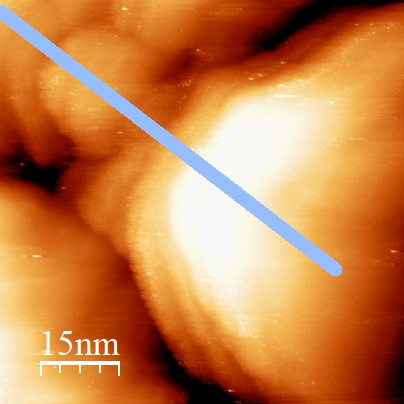
\includegraphics[scale=0.8]{Bilder/Anhang/IGain/3000_IGain_vor.jpg}
%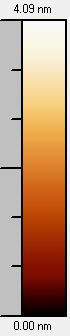
\includegraphics[scale=0.8]{Bilder/Anhang/IGain/3000_IGain_vor_Skala.jpg}
%\caption{Bild der z-Komponente bei Vermessung der Goldprobe mit einem I-Gain von 3000 in der Vorwärtsrichtung. Der Balken quer im Bild verbildlicht die Stelle, aus der das Höhenprofil entnommen wurde.}
%\label{fig:Gold_IGain_Beispiel}
%\end{figure}

\section{Ergebnisse}

\section{Fazit}


\end{document}
